
%\begin{abstract}
%When developing predictors for machine learning applications, practitioners often want to have simple and working predictors early and continue to improve them with available computational resources. 
%In this work, we propose a neural architecture search (NAS) algorithm that iteratively augments existing networks by adding shortcut connections and layers. At each iteration, we greedily select among the most cost-efficient models a parent model, and insert into it a number of candidate layers.  To learn which combination of additional layers to keep,  we simultaneously train their parameters and select the most promising candidates via feature selection techniques. The selected candidates are then jointly trained with the parent model.  Within 15 GPU-days, the proposed network growth NAS algorithm (\Petridish) can already find a model on CIFAR-10 that achieves 2.79\% error rate using 2.8M parameters.  We also transfer the model to ILSVRC2012, and it achieves 25.4\% top-1 error rate using 6.2M parameters and 810M multiply-adds. 
%Furthermore, unlike recent studies of NAS that almost exclusively focus on the small search space of repeatable network modules (cells), this work also shows that a direct search among the more general networks (macro) can also find cost-effective models when macro search is allowed to start with the same initial models as cell search does. 
%\end{abstract}

\section{Introduction}



%However, most gains have come from manually designed architectures which have inspired further improvements via careful experimentation coupled with significant experience and intuition of a skilled practitioner. Such skilled practitioners usually have significant domain knowledge of the task at hand that allows them to make rapid progress. But the fact remains that the task of designing a deep network architecture from scratch remains mostly a game of trial and error. As a consequence there has been significant effort in the community to address this issue via attempts to design algorithms that automatically find good architectures and informally referred to as AutoDNN and/or Neural Architecture Search (NAS) \cite{nas}. 

%NAS literature can be broadly categorized along three main dimensions: 1. search space 2. search procedure and 3. performance estimation strategy during the search procedure. The search space can be broadly further divided to methods that search either 1. a more general space of architectures often termed as macro-search or 2. a more constrained search space called micro or cell-search. In cell-search a good outer skeleton is often assumed. For example in image classification datasets it is common to often assume either ResNet~\citep{resnet} or DenseNet~\cite{densenet} style outer skeletons. The search can then be restricted to finding cells that fill in the slots in the outer skeleton so that the overall architecture has good performance. Cell-search is much more popular due to a number of reasons: 1. One can leverage domain knowledge of experts who have painstakingly come up with good architectures and focus the search to a smaller space. 2. Transfer to larger datasets where more capacity is often needed can be obtained by trivially stacking many cells to create larger networks. The very aspects that make cell-search attractive also prevent it from providing a truly general solution: when good outer skeletons are not available for novel domains/datasets or there is reason to believe that significant performance is left on the table, cell-search cannot be applied. By restricting the search space it is quite possible that significant performance is left on the table. On large datasets in production environments this feature is especially important. Macro-search in principle doesn't suffer from any of the above limitations but suffers from searching a much more general and larger architecture space. 


Deep neural networks have achieved state-of-the-art performance on
many large scale supervised learning tasks across many domains like
computer vision, natural language processing and audio and
speech-related tasks using architectures manually designed by skilled
practitioners using domain knowledge with experimental trial and
error.  Can we make this work for less skilled practitioners?  Is it
possible to search amongst plausible architectures in an automated
fashion to create a more automatic learning algorithm?  Neural
architecture search (NAS)~\citep{nas} algorithms attempt to
automatically find good architectures given data-sets.

We view NAS 
as a bi-level combinatorial optimization problem (as per~\citep{Liu2018DARTSDA}) where we seek both the optimal architecture 
and its associated optimal parameters.  Interestingly, this formulation 
generalizes the well-studied feature selection problem for linear prediction. 
This observation permits us to draw parallels between NAS algorithms 
and feature selection algorithms. 

In particular, a plethora of NAS works have leveraged sampling methods
including reinforcement learning~\citep{nas,NASCell,Liu2018HierNA},
evolutionary
algorithms~\citep{Real2017EvoNet,Real2018RegularizedEF,Elsken2018EfficientMN},
and Bayesian optimization~\citep{Kandasamy2018BNAS} to enumerate all
possible architectures in a guided manner.  However, interestingly, we
do not often see successes of these sampling methods for feature
selection.  Indeed, these sample-based NAS often take hundreds to
thousands of GPU-days to find good architectures, and can be barely
better than random search~\citep{Elsken2018NeuralAS}.

Another popular NAS approach is analogous to sparse optimization or
backward elimination for feature selection,
e.g.,~\citep{Liu2018DARTSDA,Pham2018EfficientNA,proxyless}.  The
approach starts with a super-graph that is the union of all possible
architectures, and learns to down-weight the unnecessary edges
gradually via gradient descent or reinforcement learning. Such
approaches drastically cut down the search time of NAS.  However,
these methods require some domain knowledge on the optimal network
size and the super-graph must fit into the GPU for efficient training.

In this work, we instead take an approach that is analogous to a
forward feature selection algorithm in order to iteratively grow
existing networks. Although forward methods such as orthogonal
matching pursuit and least-angle regression are popular in feature
selection and can often result in performance guarantees, there are
only few works in NAS~\citep{Liu2017ProgressiveNA} that take analogous
approaches.  We are interested in forward NAS approaches for multiple
reasons.  From a deployment point of view, practitioners may want to
expand their existing models when extra model complexity and training
computation become viable.  Forward methods can utilize such extra
computational resource without rebooting the training as in backward
methods and sparse optimization.  Furthermore, the iterative growth
naturally results in a spectrum of models of various complexity and
accuracy for practitioners to choose from.  Unlike backwards
approaches, forward methods need not specify a finite
search space up front making them more general and easily used.

Specifically, inspired by forward feature selection algorithms and
early neural network growth work \citep{cascadecorr}, we propose a
method (\Petridish) of growing networks from small to large, where we
opportunistically add shortcut connections in a fashion that is
analogous to applying gradient boosting to the intermediate feature
layers. To select from the possible shortcut connections, we also
exploit sparsity-inducing regularizaiton while we train the eligible
shortcuts alongside the existing networks. We experiment with it for
both the popular cell-search~\citep{NASCell}, where we seek a shortcut
connection pattern and repeat it using a manually designed skeleton
network to form an architecture, and the less popular but more general
macro-search, where shortcut connections can be freely formed.
Experimental results show \Petridish macro-search to be better than
previous macro-search NAS works on vision tasks, and brings
macro-search performance up to par with cell-search counter
to popular belief from early NAS works~\citep{nas,Pham2018EfficientNA}
that macro-search is inferior than cell-search.  \Petridish
cell-search also finds models that are more cost-efficient than those
from~\citep{Liu2018DARTSDA}, while using similar training
computation. This indicates that forward selection methods, though
currently rarely used by the NAS community, can be exploited by future
NAS algorithms.

A key tool throughout our algorithm design is amortization, where we
trade off computational costs of different operations so they are
similar up to a constant factor so as to guarantee that our approach
never wastes more than a constant factor of computation.  As an
example, training the network has a cost, as does training extensions
to the network.  By doing both simultaneously with each amortizing the
other's computational complexity we avoid significant waste
computation.

We summarize our contribution as follows.
\begin{itemize}
\item We propose an approach to increase the complexity of neural networks iteratively during training. We alternate between two phases. The first expands the model with potential shortcut connections and trains them jointly. The second phase trims the previous potential connections using feature selection and continues training the model. 
\item The proposed approach can be applied to improve a small repeatable pattern (cell), and improve the macro network architecture directly, unlike most popular approaches that only focus on cells. This opens up neural architecture search to fields where no domain knowledge of the macro structure exists. 
\item On cell-search, the proposed method finds a model that achieves 2.61\% error rate on CIFAR10 using 2.9M parameters within 5 GPU-days. 
%The model achieves \% error rate on ILSVRC2012 using M parameters and M multi-adds.
\item On macro-search, the proposed method finds a model that achieves 2.83\% error rate on CIFAR10 using 2.2M parameters within 5 GPU-days. 
%The model achieves \% error rate on ILSVRC2012 using M parameters and M multi-adds.
\item The proposed approach can warm start from existing networks, leveraging previous training results. Furthermore, it directly expands models on the lower convex hull of error rate vs. test-time computation, and is hence able to naturally produce a gallery of cost-effective models for applications to choose. 
\end{itemize}


\section{Background and References}
%\begin{itemize}
%    \item Cascade-correlation
%    \item NAS. (RL. EA. Gradient based.) 
%    \item (Micro. Macro.) 
%    \item Multi objective NAS; Pareto Front Nas 
%    \item Evaluation with few epochs vs many epochs
%    \item Incremental training, AdaNet, Boosted ResNet, Net morphism
%    \item Test~\cite{nas, NASCell, Hsu2018MONASMN, Elsken2018NeuralAS, Real2018RegularizedEF, Liu2018DARTSDA, Kandasamy2018BNAS, Pham2018EfficientNA, Liu2017ProgressiveNA}
%\end{itemize}

One of the earliest neural architecture growth was by \cite{cascadecorr} termed the ``Cascade-Correlation Learning Architecture'' (C2) which has inspired \Petridish. 
In C2, neurons of a neural network are trained iteratively. Once existing neurons are converged, C2 considers adding a candidate hidden neuron. The candidate hidden neuron before insertion to the network is connected to the input neurons and all currently existing hidden neurons. The weights of the incoming connections to this shadow neuron are optimized such that the correlation between the activations of this shadow neuron and the error at the output neurons is maximized. Then the shadow neuron is inserted into the network and its incoming weights are frozen. Its outgoing weights are then trained in the usual way. 
%There are various similarities between C2 and \Petridish which we discuss in Sec.~\ref{sec:soft_vs_hard}.
This idea of gradually expanding existing networks was also studied in a recent context~\citep{adanet, boostedresnet} through the view of boosting networks. 

The work of \citep{nas,NASCell} renewed interest in NAS in recent times. Their method uses a recursive neural network (RNN) as a controller network which is used to sample architectures. Each of these architectures are trained on separate machines and their resulting accuracies are used to update the parameters of the controller network via policy gradients~\citep{policygradient}. The majority of the time is spent in training each of the sampled architectures in parallel on independent machines. The resulting search times are generally on the order of thousands of GPU hours (See Table~\ref{tab:cifar10_search}).

\cite{Pham2018EfficientNA} introduced a much more efficient version of
this algorithm termed as Efficient Neural Architecture Search (ENAS)
where the controller samples network architectures from a large
super-graph of all possible architectures but trains them all jointly
where the weights of edges which are common amongst the sampled
architectures are shared across all of them at training time. This
leads to orders of magnitude improvement in search times but still has
the restriction that a super-graph to sample from must be constructed
apriori.

\cite{Liu2017ProgressiveNA} proposed a method which instead of using
policy gradients as in \cite{NASCell}, trains predictors on the
results of training a batch of architectures to predict top-K
architectures which are likely to do well in subsequent rounds in a
progressive manner and hence termed as Progressive Neural Architecture
Search (PNAS).

\cite{Liu2018DARTSDA} proposed a novel method based on bilevel
optimization~\citep{bilevel_opt} termed as Differentiable Architecture
Search (DARTS) which relaxes the originally discrete optimization
problem to a continuous one and maintains two sets of continuous
parameters: 1. The (architecture) parameters over the layer types and
2. The regular parameters of the network itself for each layer
type. This is optimized in an alternating fashion where first the
architecture parameters are trained alternated by the parameters of
the layers of each type. Discrete architectures are then backed out by
just selecting the architecture parameters which have the maximum
value and discarding others. DARTS achieves impressive results on
cell-search space with short search times.

\cite{Elsken2018EfficientMN, CaiPathLevel} both speed up architecture
searches by incrementally modifying models from existing
cost-effective models using evolutionary algorithms.  This work
differs from them in how the network is grown. In particular, we guide
the growth with gradient boosting on intermediate layers, instead of
using evolutionary samples for significant computational
savings.

\section{Neural Architecture Search as Optimization}
\label{sec:nas_bi_level_optimization}

Given a data sample $x$ with label $y$, a neural network architecture $\alpha$ with parameters $w$ produces 
a prediction $\hat{y}(x ; \alpha, w)$ and suffers a prediction loss $\ell(\hat{y}(x ; \alpha, w), y)$.
The expected loss is then 
\begin{align}
\mathcal{L}(\alpha, w) = \mathbb{E} _{x, y \sim \mathcal{D}} [ \ell(\hat{y}(x ; \alpha, w), y) ] 
\approx \frac{1}{|\mathcal{D}_\textrm{train}|}
   \sum _{(x, y) \in \mathcal{D}_\textrm{train}} \ell(\hat{y}(x ; \alpha, w), y) ,
\end{align}
where $\mathcal{D}$ is the true distribution of data samples, and in practice,
the loss $\mathcal{L}$ is estimated on the empirical training data $\mathcal{D}_\textrm{train}$. 
The problem of neural architectures search can be formulated as a bi-level optimization~\citep{bilevel_opt}
of both the network architecture $\alpha$ and the model parameters $w$ under the expected training loss $\mathcal{L}$ 
as follows.
\begin{align}
\min _{\alpha} \mathcal{L} (\alpha, w(\alpha)),
\quad
s.t. \quad w(\alpha) = \argmin _w \mathcal{L} (\alpha, w) 
\quad and \quad c(\alpha) \leq K,
\label{eq:bilevel_nas}
\end{align}
where $c(\alpha)$ represents the test-time computational cost of the architecture, and $K$ is some constant. 

We formalize $\alpha$ as a set of discrete decisions on which operations to include in an architecture.
Let $x_1, x_2,...,$ be intermediate layers, and $x_0 = x$ be the input. Each layer $x_i$ is a function
of the previous layers, i.e., $x_{i} = f_i ( x_0, x_1,..., x_{i-1})$ for some function $f_i$, 
though it is not necessary for $x_i$ to directly use each of the previous layers.
Each shortcut connection is defined by a triplet $(x_{j}, x_{i}, op)$, 
where $x_j$ and $x_i$ ($j < i$) represent the input and output layers, and $op$ is a unary operation such 
as conv 3x3 and max pooling 3x3. Such a shortcut results in a tensor $op(x_{j})$ that can be used directly by 
$x_i$. Shortcuts to $x_i$ are combined by a merge operation 
at $x_i$, such as averaging, summation, or concatenation in order to form $x_i$.
In this work, we set the merge operations as summation, unless we specify otherwise using ablation studies. Instead, we focus on the choice of the shortcut connections implying each $\alpha$ is an unordered collection of $(x_j, x_i, op)$.  

\subsection{Connection to Feature Selection}

Before delving into a proposed approach, we first draw an interesting connection of Eq.~\ref{eq:bilevel_nas}
to a well studied problem, feature selection for linear predictions:
\begin{align}
&\min _{\alpha} \frac{1}{2n} \Vert Y - X_{\alpha} w(\alpha) \Vert ^2 + \frac{\lambda}{2} \Vert w \Vert ^2 \\
&s.t. \quad w(\alpha) = (\frac{1}{n}X_{\alpha}^TX_{\alpha} + \lambda I)^{-1} \frac{1}{n} X_{\alpha}Y 
\quad and \quad c(\alpha) \leq K,
\label{eq:bilevel_gomp}
\end{align}
where $X \in \mathcal{R}^{n \times d}$ is the feature matrix of the $n$ samples of $d$-dimensional features,
$Y \in \mathcal{R}^n$ is the regression targets, and $X_{\alpha}$ selects the features included in $\alpha$.
We note that Eq.~\ref{eq:bilevel_nas} generalizes Eq.~\ref{eq:bilevel_gomp}, since $w(\alpha)$ solves for the 
optimal coefficient given the selected features.

This observation permits us to translate existing NAS algorithms to
feature selection algorithms as discussed in the introduction and
related work.  In contrast to most other work, ours is based on
forward selection, where feature are iteratively selected, or their
coefficients are gradually increased.  Unfortunately, common
algorithms such as Forward Regression (FR) and its approximation
Orthogonal Matching Pursuit (OMP), cannot directly be applied to the
NAS problem, because both methods require computing $w(\alpha)$ at
each architecture, with such computations taking a GPU-day on its
own. Instead, we have to consider methods that approximate $w(\alpha)$
and $\alpha$ at the same time. Fortunately, one such forward algorithm
for feature selection is Least-angle regression (LARS)~\citep{lars}.

In LARS, we compute the correlation between the residual of linear prediction and
each feature, and find the feature with the largest absolute correlation. Then we update the 
coefficient of this feature until its absolute correlation is no longer the largest.
One practical approximation of LARS is to iteratively update the coefficients of the most 
correlated feature with small steps, so that we avoid computing the line search analytically. 
Under this modification, LARS can be viewed as gradient boosting with small step sizes.
In Eq.~\ref{eq:bilevel_nas}, the gradient of the empirical loss with respect to the prediction is 
\begin{align}
\nabla _{\hat{y}} \mathcal{L} (\alpha, w) = 
\mathbb{E} _{x, y \sim \mathcal{D}} [ \nabla _{\hat{y}} \ell(\hat{y}(x ; \alpha, w), y) ].
\label{eq:nas_func_g_y}
\end{align}
Under linear prediction, this gradient becomes the residual up to a constant, 
$
\nabla _{\hat{y}} \mathcal{L} (\alpha, w) = \frac{1}{n}(X_{\alpha}w(\alpha) - Y).
$
Under linear predictions, features can be viewed as weak learners. 
Hence, the correlations between the features and the residual are
the correlations between the weak learners and the functional gradient with respect to predictions.
The selected weak learner is then the one that can match the gradient the most.  In other words, 
LARS follows gradient boosting to select weak learners.

\section{A NAS Approach from Gradient Boosting}

\label{sec:search_procedure}

\subsection{Gradient Boosting}
\label{sec:gb_review_nas}
Let $\mathcal{H}$ be a space of weak learners. 
Gradient boosting matches weak learners $h \in \mathcal{H}$ to 
the functional gradient of the loss $\mathcal{L}$ with respect to the prediction $\hat{y}$, 
i.e., $\nabla _{\hat{y}} \mathcal{L}$ in Eq.~\ref{eq:nas_func_g_y}.
The weak learner that matches the negative gradient the best, $h^*$, is added to the ensemble of learners, i.e.,
\begin{align}
h^* = \argmin _{h \in \mathcal{H}} \langle \nabla _{\hat{y}} \mathcal{L}, h \rangle.
\end{align}
Then the predictor is updated to become $\hat{y} \leftarrow \hat{y} + \eta h^*$, where $\eta$ is the learning rate.

\subsection{Gradient-Boosting-Inspired NAS}
\label{sec:gb_nas}
Following gradient boosting strictly would limit the model growth to be only at the prediction of the network, $\hat{y}$. 
Instead, this work seeks to expand the expressiveness of the network at intermediate layers, $x_1, x_2,...$, jointly.
Inspired by gradient boosting, we consider adding a weak learner $h_k \in \mathcal{H}_k$ at each $x_k$, where 
$\mathcal{H}_k$ (specified next) is the space of weak learners for layer $x_k$. 
$h_k$ helps reduce the gradient of the loss $\mathcal{L}$ with respect to $x_k$, $\nabla _{x_k} \mathcal{L}  = \mathbb{E} _{x, y \sim \mathcal{D}} [ \nabla _{x_{k}} \ell(\hat{y}(x ; \alpha, w), y) ]$.
In other words, we choose $h_k$ with 
\begin{align}
h_k = \argmin _{h \in \mathcal{H}_k} \langle h, 
\nabla _{x_k} \mathcal{L} (\alpha, w) \rangle = 
\argmin _{h\in \mathcal{H}_k} \langle h, \mathbb{E} _{x, y \sim \mathcal{D}} [ \nabla _{x_{k}} \ell(\hat{y}(x ; \alpha, w), y) ] \rangle.
\label{eq:hallu_objective}
\end{align}
Then we expand the model by adding a small step $\eta$ in the direction of $h_k$ to $x_k$.  In other words, we replace each $x_k$ with $x_k + \eta h_k$ in the original network. 
The next sections details the choice of the weak learner space, and how we learn $h_k$. 

\subsection{Search Space}
\label{sec:search_space}

\textbf{Cell-search vs. Macro-search.}
The early architecture searches~\citep{nas,Real2017EvoNet} typically allow any layer to connect to any other layer. 
This is often referred to as macro-search. 
However, as a number of works \citep{NASCell,Real2018RegularizedEF,Pham2018EfficientNA} showcase that 
a more restricted search, cell-search, leads to better models, the community has almost abandoned macro-search.
As illustrated in Fig.~\ref{fig:cell_vs_macro_search}, in a cell-search, the search algorithm search for a local connection pattern called cell, 
such as the residual unit in a ResNet~\citep{resnet}. The cells instruct how neighboring layers are connected, and 
we apply these patterns in a human defined outer structure to form the final network. 
For example, the outer structure may be a straight-forward feed-forward network that contains 
information of the total number of cells and where down-sampling happens. 
In contrast, in a macro-search, the search algorithm is allowed to connect any layer to another, 
so that there is no predefined outer structure, and there may not be repeatable patterns that can be considered as cells. 

\begin{figure}
\centering
\subfloat[]{
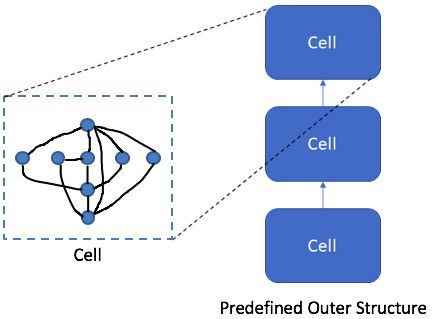
\includegraphics[keepaspectratio,height=0.3\textwidth]{\NASDIR/img/cell_search.png}
}
~
\subfloat[]{
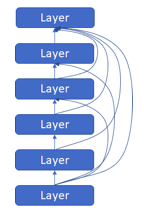
\includegraphics[keepaspectratio,height=0.3\textwidth]{\NASDIR/img/macro_search.png}
}
\caption{(a) Cell-search applies found cells to a predefined outer structure. (b) Macro-search allows any connection. }
\label{fig:cell_vs_macro_search}
\end{figure}

In this work, we revisit macro-search. 
For a fair comparison between macro-search and cell-search, 
we set the only difference between the two to be whether the connection pattern is repeated. 
Specifically, both start with the same initial seed model, which is a network built with simple cells.
Both searches add weak learners at the same locations and at the same rate: one weak learner is always added to the end output of each cell per growth iteration.  Cell-search adds the same connection pattern to each cell while macro-search allows different patterns. 
The space of the weak learners, which we detail next, is the same for both. 



\textbf{Weak Learner Space $\mathcal{H}$.}
Given an intermediate layer $x_{k}$ to expand at, its associated weak learner space $\mathcal{H}_{k}$ is defined by four terms: the possible inputs, the
possible unary operations on the inputs, a merge operation to combine the results, and the maximum number of inputs. 
Following~\citep{NASCell,Real2018RegularizedEF,Liu2018DARTSDA}, we limit weak learners to only take input from layers within the same cell or from the output layers of the previous 
two cells. 
The eligible unary operations are dependent on data-set. Following~\citep{Liu2018DARTSDA}, seven operations are eligible for vision tasks:  
separable conv 3x3 and 5x5, dilated conv 3x3 and 5x5, max and average pooling 3x3, and identity. Following~\citep{NASCell,Real2018RegularizedEF}, the separable conv is 
repeated twice. The outputs of the unary operations are of the same shape 
as the output location $x_k$. 
Let the collection of eligible unary operations be $\texttt{Op}$.
We determine through an ablation study in Sec.~\ref{sec:sum_vs_cat_proj} how to merge the unary operations into a weak learner. For vision tasks, we found 
concatenation of the operations followed by a projection to reduce the filter size works the best. 
The maximum number of inputs is also data-set dependent, and for vision tasks, we set it to be $I_{max} = 3$, which we choose from ablation studies in experiments.
Then the weak learner space $\mathcal{H}_{k}$ for a layer $x_{k}$ is formally 
\begin{align}
\mathcal{H}_{k} = \{ \texttt{cat\_proj}( op_1(z_1), ..., op_{I_{max}}(z_{I_{max}})) : z_1, ..., z_t \in \texttt{In}(x_{k}), op_1, ..., op_{I_{max}} \in \texttt{Op}  \},
\end{align}
where $\texttt{In}(x_{k})$ is the collection of eligible input layers.
Fig.~\ref{fig:cell_search_space} shows an example of a weak learner in the above space. 
\begin{figure}
\centering
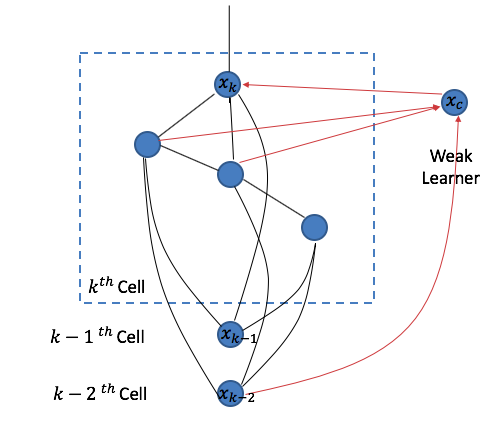
\includegraphics[keepaspectratio,height=0.4\textwidth]{\NASDIR/img/cell_search_space.png}
\caption{An example weak learner $x_c$ from the search space $\mathcal{H}_k$.}
\label{fig:cell_search_space}
\end{figure}


\textbf{Additional Search Space Details.}
For the vision tasks, the initial model for both macro and cell-search is a modified ResNet~\citep{resnet}, where we replace each 3x3 convolution with a 3x3 separable convolution. This is one of the simplest seeds within the search space of existing literature~\citep{NASCell,Pham2018EfficientNA,Liu2018DARTSDA}.  Following ~\citep{NASCell}, we have six regular cells for each of the three scales of feature maps during training of the final found architectures, 
but have three regular cells per scale during search. Similarly, we have an initial channel size of $F=32$ during final training and $F=16$ during search. 
A transition cell is in between each neighboring resolutions, and it also starts as a modified residual unit. 
When we transfer the model to larger data-sets that require more than three resolutions, we use transition cells to first down-sample the image height and width to be no greater than 32 and then apply the found model. In macro-search, where no transition cells are specifically learned, we again use the the modified ResNet cells for initial transition in the transferred model.


\subsection{Joint Weak Learning}
\label{sec:candidate_init_and_select}

\begin{algorithm}[t]
\begin{algorithmic}[1]
\STATE \textbf{Input}: 
(1) $L_x$, the list of layers in the current model (macro-search) or current cell (cell-search) in topological order;
(2) $\texttt{is\_out}(x)$, whether we can expand at $x$;
(3) $\lambda$, hyper parameter for selection shortcut connections. 
\STATE \textbf{Output}: (1) $L'_x$, the modified $L_x$ with weak learners $x_c$; 
(2) $L_c$, the list of $x_c$ created;
(3) $\ell_{extra}$, the additional training loss.

\STATE $L'_x \leftarrow L_x$
\STATE $L_c \leftarrow \text{empty list}$
\STATE $\ell_{extra} \leftarrow 0$ 
\FOR{$x_k$ in enumerate($L_x$)}
    \IF { not \texttt{is\_out}($x_{k}$)}
        \STATE continue
    \ENDIF
    \STATE Compute the eligible inputs $\text{In}(x_{k})$, and index them as $z_1,...,z_I$.

    %\STATE Initialize $\alpha_{i,j}$ randomly from Gaussian. 
    %\STATE Initialize parameters in $op_j(x_{in,i})$. 
    \STATE $x_c \leftarrow \sum _{i=1}^I \sum _{j=1}^J  \alpha^k_{i,j}op_j(\stopgradient (z_i))$.
    \label{algline:add_sg}
\STATE Insert the layer $x_c$ right before $x_{k}$ in $L'_x$.
\STATE $\ell_{extra} \leftarrow \ell_{extra} + \lambda \sum _{i=1}^I \sum _{j=1}^J |\alpha^k_{i,j}|$.
\STATE Append $x_c$ to $L_c$.
\STATE Modify $x_{k}$ in $L'_x$ so that $x_{k} \leftarrow x_{k} + \stopforward (x_c)$.
\label{algline:add_sf}
\ENDFOR
\end{algorithmic}
\caption{\Petridish .initialize\_candidates}
\label{alg:candidate_init}
\end{algorithm}

\begin{algorithm}[t]
\begin{algorithmic}[1]
\STATE \textbf{Inputs}: (1) $L'_x$, the list of layers of the model in topological order;
(2) $L_c$, list of selection modules in $L'_x$;
(3) $\alpha^k_{i,j}$, the learned weights of the each $x_c$. 
\STATE \textbf{Output}: A modified $L'_x$ with selected operations.
\FOR{$x_c$ in $L_c$}
    \STATE Let $A = \{\alpha^{k}_{i,j}: i = 1,..., I, j = 1,..., J\}$  be the weights of operations in $x_c$.
    \STATE Sort $\{ |a| : a \in A \}$, and let the operations associated with the largest $I_{max}$ value be $op_1, ..., op_{I_{max}}$.
    \STATE Replace $x_c$ with $\text{proj}(\text{concat}(op_1, ..., op_{I_{max}}))$ in $L'_x$.
\ENDFOR
\STATE Replace all $\stopforward (\cdot)$ and $\stopgradient (\cdot)$ with identity in $L'_x$.
\end{algorithmic}
\caption{\Petridish .finalize\_candidates}
\label{alg:candidate_select}
\end{algorithm}


Given an intermediate layer $x_{k}$ to expand at, we have $I = |\texttt{In}(x_{k})|$ possible input layers and $J = |\texttt{Op}|$ possible operations.
Hence, there are $\binom{IJ}{I_{max}}$ possible weak learners
in the space $\mathcal{H}_{k}$, and it is computationally expensive to train each weak learner individually. 
Inspired by the parameter sharing works in NAS~\citep{Pham2018EfficientNA,Liu2018DARTSDA} and model compression in neural networks~\citep{huang2017condensenet},
we propose to jointly train the weak learners in the union of them, 
and at the same time learn to select the shortcut connections.  This process effectively amortizes the search through all weak learners against other weak learners so the computational cost is only a constant factor worse than for the chosen weak learner.

Algorithm~\ref{alg:candidate_init} describes the proposed approach to train the weak learners. 
For now, let us assume the boolean variable
This means that weak learning does not affect the parameters of the current model. 
Fig.~\ref{fig:x_c_select_sf_sg} illustrates the weak learning modification to the current network. 

\begin{figure}[ht]
\centering
\subfloat[]{
    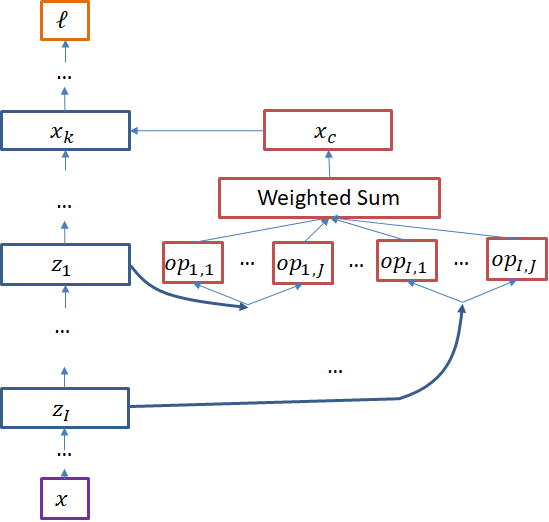
\includegraphics[width=0.44\textwidth, keepaspectratio]{\NASDIR/img/x_c_select.png}
    \label{fig:x_c_select}}
    ~
\subfloat[]{
    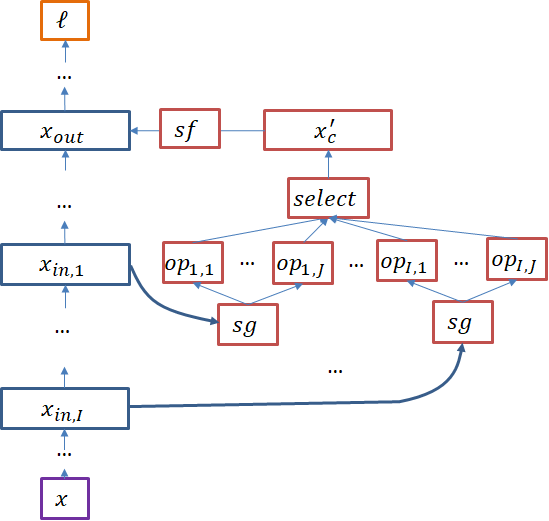
\includegraphics[width=0.44\textwidth, keepaspectratio]{\NASDIR/img/x_c_select_sf_sg.png}
    \label{fig:x_c_select_sf_sg}}
    \caption{Training of a weak learner $x_c$, so that it can (a) and cannot (b) affect the current model.}
\end{figure}

\textbf{Combining Weak Learners.} During joint weak learning, we combine all shortcut connections to 
$x_k$ in a weighted sum as follows. 
\begin{align}
    x_c = \sum _{i=1}^I \sum_{j=1}^J \alpha_{i,j} op_j(z_i),
    \label{eq:x_c_select}
\end{align}
where $op_j \in \texttt{Op}$ and $z_i \in \texttt{In}(x_k)$ enumerate all possible operations and inputs, and $\alpha_{i,j} \in \mathbb{R}$ is the weight of the shortcut $op_j(z_i)$. 
The next paragraphs explain how we simultaneously train and select the shortcuts to form a weak learner for $x_k$. 

\textbf{$L1$-regularization.} Each $op_j(z_i)$ is normalized with batch-normalization to have zero mean and unit variance in expectation, so $\alpha_{i,j}$ reflects 
the importance of the operation.
To learn the most important operations, we apply $L1$-regularization~\citep{lasso} on the weight vector $\vec{\alpha}$ to encourage sparsity, i.e.,
we add the following loss during the fitting of $x_c$,  
\begin{align}
    \lambda \Vert \vec{\alpha} \Vert_1 = 
    \lambda \sum_{i=1}^I \sum _{j=1}^J | \alpha _{i,j} |,
    \label{eq:x_c_select_loss}
\end{align} 
where $\lambda$ is a hyperparameter. $L1$-regularization, known as Lasso, induces sparsity in the parameter and is widely used for feature selection. It has also been successfully applied to model compression of neural networks such as in~\citep{huang2017condensenet}.


\textbf{Weak learning.} 
The goal of weak learning is to match $x_c$ with the negative gradient of the loss with respect to the layer $x_{k}$, i.e., 
we minimize 
\begin{align}
   \langle \nabla_{x_{k}} \mathcal{L}, x_c \rangle =  
   \langle \nabla_{x_{k}} \mathcal{L}, \sum _{i=1}^I \sum_{j=1}^J \alpha_{i,j} op_j( \stopgradient( z_i ) ) \rangle,
    \label{eq:x_c_linear_loss}
\end{align}
where $\stopgradient$ is short for stop-gradient, an operation which treats each $z_i$ as a constant, so that the optimization of weak learners does not 
affect the current network. Mathematically, $\stopgradient(x) = x$ during forward, and has zero gradient with respect to $x$ during backward.

We add the loss~\ref{eq:x_c_linear_loss} implicitly to the overall
objective on line~\ref{algline:add_sf}.  A naive implementation adds
the loss in Eq.~\ref{eq:x_c_linear_loss} to the additional
$\ell_{extra}$, and backpropagates the network while only updating
parameters in the weak learners $x_c$.  However, this requires recording the intermediate gradients $\nabla _{x_{k}} \mathcal{L}$
during training.  Interestingly, this can be avoided as described in Algorithm~\ref{alg:candidate_init}.  Specifically, on
line~\ref{algline:add_sf}, we replace the layer $x_k$ with $x_k +
\stopforward(x_c)$, where $\stopforward(x_c) = x_c -
\stopgradient(x_c)$, so that $\stopforward(x_c) = 0$ during forward,
and has gradient of identity with respect to $x_c$. As a result, for
any parameter $\theta$ in weak learner $x_c$ for intermediate layer
$x_k$, its gradient during the backpropagation is
\begin{align}
\nabla_{\theta} \mathcal{L} &= \nabla _{x_k + \stopforward(x_c)} \mathcal{L} \nabla _{x_c} \stopforward(x_c) \nabla _{\theta} x_c = \nabla _{x_k}\mathcal{L} \nabla _{\theta} x_c = \nabla_{\theta} \langle \nabla_{x_{k}} \mathcal{L}, x_c \rangle.
\end{align}
This is the same as the gradient of the loss in
Eq.~\ref{eq:x_c_linear_loss} with respect to $\theta$.  Hence,
exploiting $\stopforward$ and $\stopgradient$ operations on
line~\ref{algline:add_sf} and line~\ref{algline:add_sg}, we can
optimize both the current network and the weak learners at the same
time without the weak learners affecting the network achieving
amortization between network learning and weak learner learning.
Furthermore, we do not force the training procedure to record
$\nabla_{x_k} \mathcal{L}$ explicitly.

\textbf{Warm-start.} After appending the weak learners to an existing trained model, we warm-start the training with the parameters
of the existing model, and initialize the weak-learner parameters randomly. Leveraging these existing model parameters, 
we can potentially spend fewer epochs per model, because we only need to fit the weak learners, which are
shallow networks.


\subsection{Weak Learner Finalization}
\label{sec:candidate_finalize}

\begin{figure}[t]
\centering
    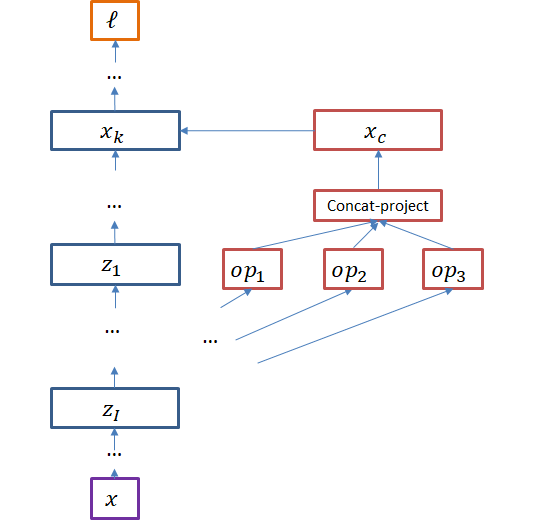
\includegraphics[width=0.44\textwidth, keepaspectratio]{\NASDIR/img/x_c_select_final.png}
    \caption{Weighted sum is replaced with concat-projection, when the top operations are chosen. Any $\stopforward$ or $\stopgradient$ are also removed.}
    \label{fig:x_c_select_final}
\end{figure}

In Algorithm~\ref{alg:candidate_select}, we finalize the weak learners. Since the weights $\alpha_{i,j}$ convey the importance of the associated shortcuts, we select for each $x_c$ of Eq.~\ref{eq:x_c_select} the top $I_{max}$ shortcuts according to the absolute value of $\alpha_{i,j}$, and merge them to form the selected weak learner. The other operations are removed. 
We train the finalized model for a few epochs, warm-starting with the parameters from the weak learning phase. 
Although we train and select the shortcuts in a weighted sum, we found through ablation study in Sec.~\ref{sec:sum_vs_cat_proj} that for vision tasks, the found models are more cost-effective if we merge the $I_{max}$ selected shortcuts with concatenation-projection, as illustrated in Fig.~\ref{fig:x_c_select_final}. Existing NAS works~\citep{NASCell,Real2018RegularizedEF,Pham2018EfficientNA,Liu2018DARTSDA} have a similar set-up, where intermediate layers within cells are concatenated, and the concatenation is immediately projected when it is an input to other cells. 

\subsection{Utilizing Parallel Workers}
\label{sec:parent_choice}

The proposed iterative architecture growth may be noisy 
due to the randomness during training of weak learners and 
the expanded models. By leveraging parallel workers, we 
can explore multiple growths to find more cost-effective models. 
The parallel workers can share knowledge and expand from any searched models, 
with this section describing their sampling procedure.

We maintain the lower convex hull of the performance of the 
searched models on the validation error versus test-time computation 
graph. The models on the hull are the most cost-efficient, 
because no mixture of other searched models is both more accurate and less expensive
than any of them. To choose one model on the hull, we enter a while-loop
iterating from the most accurate model that is within the computational  
budget $K$ to the least accurate on the hull, 
and exit the loop with a model $m$ with probability $1/(n(m) + 1)$, 
where $n(m)$ is the number of times that model $m$ has already been selected. 
This is because the next child model expanded from $m$ is the best among the children with probability
$1/(n(m) + 1)$, assuming the children are uniformly drawn. 
We also favor the more accurate models as it is often more difficult to 
improve an already accurate model. In practice, we explore few 
models in total $(<50)$, so that the effect of different sampling on the hull 
is not clear given the limited search samples. 


\section{Selected Empirical Highlights}
\label{sec:nas_experiment}

%%%%%%%%%%%%%%%%%%%%%%%% 
% Experimental questions
%%%%%%%%%%%%%%%%%%%%%%%%
%\subsection{Experimental questions}
%\begin{enumerate}
%\item 
%\end{enumerate}


%%%%%%%%%%%%%%%%%%%%%%%% 
% Data-sets
%%%%%%%%%%%%%%%%%%%%%%%%

%%%%%%%%%%%%%%%%%%%%%%%% 
% Eval metric
%%%%%%%%%%%%%%%%%%%%%%%%
%\subsection{Evaluation Metrics}

%\begin{enumerate}
%    \item For fixed search space and training parameters, we can 
%    compare the best found model validation error after the same number of 
%    models are trained.
    %\item For a more general comparison among search algorithms, we plot the curves of the best validation error versus FLOPs spent on training. Then the lower curves represent algorithms that find the most accurate models faster.
    %\item While the previous two metrics focus on how fast the search can find the most accurate models, they do not consider the cost-efficiency of the searched models. To evaluate the cost-efficiency, we represent the cost-efficiency of searched models by the lower convex hull of validation error versus model computational cost, measured in FLOPs. The more close the hull is to the origin, the more cost efficient the found models are. We can compare algorithms by comparing their performance convex hulls. 
%\end{enumerate}


%%%%%%%%%%%%%%%%%%%%%%%% 
% Parent choice Experiment
%%%%%%%%%%%%%%%%%%%%%%%%

Following~\citep{NASCell}, we first report the search results on CIFAR-10~\citep{cifar} and the model transfer result to ImageNet~\citep{ILSVRC15}. Then we report ablation studies on hyper parameters of \Petridish. 

%%%%%%%%%%%%%%%%%%%%%%%% 
% Visual Recognition Data-sets
%%%%%%%%%%%%%%%%%%%%%%%%
\subsection{Search Results on CIFAR10}
\label{sec:experiment_cifar10_search}

\textbf{Set-up.}
We first apply the proposed algorithm to search for architectures on CIFAR-10~\citep{cifar}. During search, we use a fixed set of 45000 training images for training, and 5000 for validation. Both weak learner initialization and finalization are trained for 80 epochs, with a batch size 32 and a learning rate that decays from 0.025 to 0 in cosine decay~\citep{cosine_lr}. We apply drop-out~\citep{larsson2016fractalnet} and cut-out~\citep{cutout} during search. The final found model is trained from scratch using the same parameters, except that it trains on all 50000 training images, and spends 600 epochs. 
Following~\citep{NASCell,Liu2018DARTSDA}, we search on a shallower and slimmer version of the network, which has $N=3$ normal cells per feature map resolution and $F=16$ initial filter size. The final training is instead on a network with $N=6$ and $F=32$. Since \Petridish macro-search is simply cell-search binding the cells to be the same, we transform macro-search results on $N=3$ to models with $N=6$ by repeating each normal cell twice. 
The initial seed model is trained for 200 epochs, and all subsequent children models with or without weak learners are trained for 80 epochs each, warm starting from their parent models' parameters. 

\textbf{Search Results.} 
Table~\ref{tab:cifar10_search} depicts the test-errors, model parameters, and search computation of the proposed methods along with many state-of-the-art methods.
\Petridish cell search finds a model with 2.61\% error rate with 2.5M parameters, in 5 GPU-days, which is at state-of-the-art level. \Petridish macro search finds a model that achieves 2.83\% error rate using 2.2M parameters in the same search computation. This is significantly better than any previous macro search results, 
and showcases that macro search can find cost-effective architectures that are previously only found through cell search. 

\textbf{Importance of initial models.}
Table~\ref{tab:cifar10_search} also showcase the impact of initial models to the final results of architecture search. This is an important topic, because existing literature has been moving away from macro architecture search, as early works~\citep{NASCell,Pham2018EfficientNA,Real2018RegularizedEF} have shown that cell search results tend to be superior to those from macro search. However, this result may be explained by the superior initial models of cell search: the initial model of \Petridish is one of the simplest models that any of the listed cell search methods would propose and evaluate, and it already achieves 4.6\% error rate using only 0.4M parameters, a result is on-par or better than any other macro search results. 


\begin{table*}[t]
    \centering
    \caption{Comparison against state-of-the-art recognition results on CIFAR-10. Results marked with $\dagger$ are not trained with cutout. The first block represents approaches for macro-search. The second block represents approaches for cell-search. 
    }
    \begin{tabular}{l|cccc}
    \hline
\multirow{ 2}{*}{\textbf{Method} }
        &  \textbf{\# params} 
        &  \textbf{Search } 
        &  \textbf{Test Error } \\
        &  (mil.)
        &  (GPU-Days)
        &  (\%)\\
\hline
\citet{nas}$^{\dagger}$
    &  7.1 &  1680+ &  4.47  \\
\citet{nas} + more filters$^{\dagger}$
    &  37.4 &   1680+ &  3.65   \\
\citet{Real2017EvoNet}$^{\dagger}$
    &  5.4 &   2500 &  5.4  \\
ENAS macro~\citep{Pham2018EfficientNA}$^{\dagger}$
    &  21.3 &  0.32 &  4.23 \\
ENAS macro + more filters$^{\dagger}$
    &  38 &   0.32 &  3.87 \\
Lemonade I~\citep{Elsken2018EfficientMN}
    &  8.9 &    56 &  3.37 \\
\hline
\Petridish initial model ($N=6$, $F=32$)
    & 0.4 &  -- & 4.6 \\
%\Petridish macro without DropPath
%    & 3.1 & 6 & 3.38 \\
\textbf{\Petridish macro} 
    & \textbf{2.2} & 5 & \textbf{2.83} \\
%\Petridish macro (start at $N$=3, $F$=32)
%    & 2.7 & 18 & 3.44 \\
\hline \hline
NasNet-A~\citep{NASCell}
    &  3.3 &    1800 &  2.65   \\
AmoebaNet-A~\citep{Real2018RegularizedEF}
    &  3.2 &  3150 &  3.3  \\
AmoebaNet-B~\citep{Real2018RegularizedEF} 
    &  2.8 &   3150 &  2.55 \\ 
PNAS~\citep{Liu2017ProgressiveNA}$^{\dagger}$
    &  3.2 &  225 &  3.41 \\
Heirarchical NAS~\citep{Liu2018HierNA}$^{\dagger}$
    &  15.7 &    300 &  3.75 \\ 
ENAS cell~\citep{Pham2018EfficientNA}
    &  4.6 &  0.45 &  2.89 \\ 
ENAS cell~\citep{Pham2018EfficientNA}$^{\dagger}$
    &  4.6 &  0.45 &  3.54 \\ 
Lemonade II~\citep{Elsken2018EfficientMN}
    &  3.98 &  56 &  3.50 \\
Darts~\citep{Liu2018DARTSDA}
    &  3.4 &   4 &  2.83 \\ 
Darts random~\citep{Liu2018DARTSDA}
    & 3.1 & -- & 3.49 \\
\citet{CaiPathLevel} 
    & 5.7 &  8  & 2.49 \\
\citet{NAONet}$^{\dagger}$
    & 3.3 & 0.4 & 3.53 \\
PARSEC \citep{parsec}
    & 3.7  & 1 & 2.81 \\
\hline
\textbf{\Petridish cell}
    & \textbf{2.5} & 5 & \textbf{2.61} \\
%\Petridish cell + more filters
%    & 3.5 & 6 & 3.05 \\
\hline
    \end{tabular}
    \label{tab:cifar10_search}
\end{table*}


\subsection{Transfer to ImageNet}
\label{sec:experiment_vision_transfer}


\begin{table*}[t]
    \centering
    \caption{ILSVRC2012 transfer results. \Petridish uses \petridishhard and the concat-projection (CP) modification by default. 
    }
    \begin{tabular}{l|cccc}
    \hline
\multirow{ 2}{*}{\textbf{Method} }
        &  \textbf{\# params} 
        &  \textbf{\# multi-add}
        &  \textbf{Search}
        &  \textbf{top-1 Test Error } \\
        &  (mil.)
        &  (mil.)
        &  (GPU-Days)
        &  (\%)\\
\hline
Inception-v1 (Szegedy et al., 2015)
    & 6.6 & 1448 & -- & 30.2 \\
MobileNetV2 (Sandler et al., 2018)
    & 6.9 & 585 & -- & 28.0 \\
\hline
NASNet-A (Zoph et al., 2017) 
    & 5.3 & 564 & 1800 & 26.0 \\
NASNet-B (Zoph et al., 2017) 
    & 5.3 & 488 & 1800 & 27.2 \\
AmoebaNet-A (Real et al., 2018)
    & 5.1 & 555 & 3150 & 25.5 \\
Path-level (Cai et al., 2018)
    & -- & 588 & 8.3 & 25.5 \\
PNAS (Liu et al., 2017a)
    & 5.1 & 588 & 225  & 25.8 \\
DARTS (Liu et al., 2019)
    & 4.9 & 595 & 4    & 26.9 \\
SNAS \citep{snas}
    & 4.3 & 522 & 1.6 & 27.3 \\
Proxyless \citep{proxyless}
    & 7.1 & 465 & 8.3 & 24.9 \\
PARSEC \citep{parsec}
    & 5.6 & -- & 1  & 26.0 \\
\hline
\textbf{\Petridish macro} (F=44) %828
    & 4.3 & 511 & 5 & 28.5 \\
\hline
\textbf{\Petridish cell} (F=40) %1172
	& 3.2 & 500 & 5 & 27.0 \\
\textbf{\Petridish cell} (F=44) %1180 
    & 4.8 & 598 & 5 & 26.0 \\
\hline
\end{tabular}
\label{tab:imagenet_compare}
\end{table*}


We focus on the mobile setting for the model transfer results on ILSVRC~\citep{ILSVRC15}. 
Following~\citep{NASCell}, we use 224x224 cropped input images, and apply to them a 3x3 conv with $F / 4$ filters and stride of 2. Then we apply two transition cells to convert the feature map to 28x28 and $F$ filters. For macro-search results, we apply the transition cell in the seed model, i.e., residual units from~\citep{resnet} where conv is replaced with separated conv. We then treat the resulting tensor as the input image for the found architectures. 
We follow~\citep{Liu2018DARTSDA} to choose the training hyper parameters: we train for 250 epochs with batch size 128, weight decay $3*10^{-5}$, and initital SGD learning rate of 0.1 (decayed by a factor of 0.97 per epoch). 

The top-1 error rate, the number of model parameters and the test-time computational cost in terms of mult-adds are shown in Table~\ref{tab:imagenet_compare}.  The \Petridish cell-search model achieves 26.0\% error rate using 4.8M parameters and 598M multiply-adds, which is on par with state-of-the-art results listed in the second block of Table~\ref{tab:imagenet_compare}. By utilizing feature selection techniques to evaluate multiple model expansions at the same time, \Petridish is able to find models faster by one or two orders of magnitude than early methods that train models independently, such as NASNet~\citep{NASCell}, AmoebaNet~\citep{Real2018RegularizedEF}, and PNAS~\citep{Liu2017ProgressiveNA}.  
In comparison to super-graph methods such as DARTS~\citep{Liu2018DARTSDA}, \Petridish cell-search sacrifices about a factor of four search speed for the flexibility to grow from existing models. 

The \Petridish macro-search model achieves 28.5\% error rate using 4.3M parameters and 511M multiply-adds, a comparable result to the human-designed models in the first block of Table~\ref{tab:imagenet_compare}. To the best of our knowledge, this is one of the first successful result to transfer macro-search results on CIFAR to ImageNet, showing that macro-search results can be transferred. 
However, we do observe a gap in error rates between \Petridish macro and cell search both during search and the model transfer. This suggests that the larger macro search space is more difficult. 

As \Petridish gradually expand existing models, we naturally receive a gallery of models of various computational costs and accuracy. Figure~\ref{fig:imagenet_convexhull} showcases the found models by \Petridish with $F=44$. We removed the seed model and points that are no longer on the lower convex hull. 

\begin{figure}
    \centering
    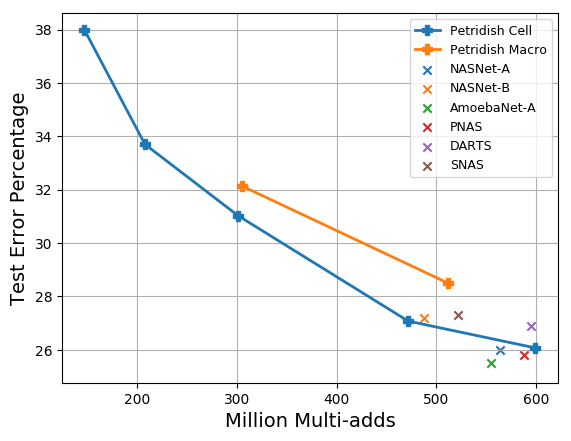
\includegraphics[width=0.5\textwidth,keepaspectratio]{\NASDIR/img/final_CH_keys_951_965.png}
    \caption{The performance convex hull of the found models by \Petridish on ILSVRC. \Petridish models are of parameter $N=6$ and $F=44$.}
    \label{fig:imagenet_convexhull}
\end{figure}

\subsection{Search Space: Direct versus Proxy}
This section provides an ablation study on a common theme of recent 
neural architecture search works, where the search is conducted on a proxy space of small and shallow models, with results transferred to 
larger models later. In particular, since \Petridish uses iterative growth, it need not consider the complexity of a super graph containing all possible models. Thus, \Petridish can be applied directly to the final model setting on CIFAR-10, where $N=6$ and $F=32$. However, this implies each model takes about eight times the computation, and may introduce extra difficulty in convergence. Table~\ref{tab:direct_vs_proxy} shows the transfer results of the two approaches to ILSVRC.  We see that using a proxy not only results in a model with about 1\% less errors, but also takes about one third of the search time, confirming that on image tasks the proxy approach is effective. 

\begin{table}[t]
    \centering
    \begin{tabular}{l|cccc}
    \hline
\multirow{ 2}{*}{\textbf{Method} }
        &  \textbf{\# params} 
        &  \textbf{\# multi-add}
        &  \textbf{Search}
        &  \textbf{top-1 Test Error } \\
        &  (mil.)
        &  (mil.)
        &  (GPU-Days)
        &  (\%)\\
    \hline
    \textbf{\Petridish cell proxy} (F=44) %1180 
        & 4.8 & 598 & 5 & 26.0 \\
    \textbf{\Petridish cell direct} (F=40) %841
        & 4.4 & 583 & 15.3 &  26.9 \\
    \hline
    \end{tabular}
    \caption{Search space comparison between the direct space of $N=6$ and $F=32$ and the proxy space of $N=3$ and $F=16$ by evaluating their best mobile setting models on ILSVRC.}
    \label{tab:direct_vs_proxy}
\end{table}



\subsection{Weak Learner Space: Weighted Sum versus Concatenation-Projection}
\label{sec:sum_vs_cat_proj}


\begin{table}[t]
    \centering
    \caption{ILSVRC2012 transfer results. 
    	Ablation study on the choice of weighted-sum (WS), concat-projection at the end (CP-end), or the \Petridish default merge operation in finalized weak learners.
    	The searches were done with parameter initial channel $F=32$ and s number of regular cells per resolution of $N=6$. 
    }
    \begin{tabular}{l|cccc}
    \hline
\multirow{ 2}{*}{\textbf{Method} }
        &  \textbf{\# params} 
        &  \textbf{\# multi-add}
        &  \textbf{Search}
        &  \textbf{top-1 Test Error } \\
        &  (mil.)
        &  (mil.)
        &  (GPU-Days)
        &  (\%)\\
\hline
WS macro(F=48) %808
    & 5.9 & 756 & 29.5 & 32.5\\
CP-end macro (F=36) %845
    & 5.4 & 680 & 29.5 & 29.1 \\
{\Petridish macro} (F=32) %828
    & 4.9 & 593 & 27.2 & 29.4 \\
\hline
WS cell (F=48) %810
    & 3.3 & 477 & 22.8 & 32.7\\
CP-end cell  (F=44) %848
    & 4.7 & 630 & 22.8 & 27.2 \\
\textbf{\Petridish cell} (F=40) %841
    & 4.4 & 583 & 15.3 &  26.9 \\
\hline  
\end{tabular}
\label{tab:imagenet_ws_vs_cp}
\end{table}


After selecting the shortcuts in Sec.~\ref{sec:candidate_finalize}, we concatenate them and project the result with 1x1 conv so that the result can be added to the output layer $x_{out}$. 
Here we empirically justify this design choice through consideration of two alternatives.  
We first consider applying the switch only to the final reported model.  In other words, instead of using concat-project as the merge operation during search we switch all weak learner weighted-sums to concat-projections in the final model, which are trained from scratch to report results.  We call this variant CP-end.  Another variant where we never switch to concat-projection is called WS. Since concat-projection incurs additional computation to the model, we increase the channel size of WS variants so that the two variants have similar test-time multiply-adds for fair comparisons. The default \Petridish option is switching the weak learner weighted-sums to concat-projections each time weak learners are finalized.  We compare WS, CP-end and \Petridish on the transfer results on ImageNet in  Table~\ref{tab:imagenet_ws_vs_cp}, and observe that \Petridish achieves similar or better prediction error using less test-time computation and training-time search. 


\subsection{Weak Learner Space: Number of Merged Operations}
\label{sec:experiment_number_operations}
As we initialize all possible shortcuts during weak learning, we need decide $I$, the number of them to select for forming the weak learner. On one hand, adding complex weak learners can boost performance rapidly. On the other, this may add sub-optimal weak learners that hinder future growth. We test the choice of $I=2,3,4$ during search. We run with each choice five times, and take the average of their most accurate models that take under 60 million multi-adds on the CIFAR model with $N=3$ and $F=16$. Models in this range are chosen, because their transferred models to ILSVRC can have 600 million multi-adds with standard setups of~\citep{NASCell}, and hence, they are natural candidate models for ILSVRC mobile setting. Table~\ref{tab:cifar10_search_choose_i} reports the test error rates on CIFAR10, and we see that $I=3$ yields the best results. 



\begin{table}[t]
    \centering
    \caption{Test error rates on CIFAR-10 by models found with different weak learner complexities.
    }
    \begin{tabular}{c|c}
    \hline
    Number of Shortcuts & Average Lowest Error Rate \\
    \hline
    $I=2$ & 3.08  \\ %1195 
    $I=3$ & 2.68 \\  %1196
    $I=4$ & 2.93 \\ %1197
    \hline
    \end{tabular}
    \label{tab:cifar10_search_choose_i}
\end{table}


\subsection{Weaker Learner Training: Joint versus Isolated training with Parent Model}
\label{sec:experiment_soft_vs_hard}

\begin{table}[t]
    \centering
    \caption{ILSVRC2012 transfer results. 
    	Ablation study on the choice of \petridishsoft and \petridishhard for training the weak learners. 
    	The search were with parameter initial channel $F=32$ and number of regular cell per resolution $N=6$. 
    }
    \begin{tabular}{l|cccc}
    \hline
\multirow{ 2}{*}{\textbf{Method} }
        &  \textbf{\# params} 
        &  \textbf{\# multi-add}
        &  \textbf{Search}
        &  \textbf{top-1 Test Error } \\
        &  (mil.)
        &  (mil.)
        &  (GPU-Days)
        &  (\%)\\
\hline
\Petridish \petridishsoft cell (F=32) %843,842,833,834
    & 4.0 & 546 & 20.6 & 32.8 \\
\textbf{\Petridish cell} (F=40) %841
    & 4.4 & 583 & 15.3 &  26.9 \\
\hline
\end{tabular}
\label{tab:imagenet_soft_vs_hard}
\end{table}


An interesting consideration is whether to stop the influence of the
weak learners to the models during the weak learning.  On one hand, we
eventually want to add the weak learners into the model and allow them
to be backpropagated together to improve the model accuracy.  On the
other hand, the introduction of untrained weak learners to trained
models may negatively affect the training. Furthermore, the models may
develop dependency on weak-learner shortcuts that are not selected,
which can also negatively affect the future models.  To study the
effects through an ablation study, we replace the occurrence of
$\stopforward$ and $\stopgradient$ with identity in
Algorithm~\ref{alg:candidate_init}, so that the weak learners are
directly added to the models, as illustrated in
Fig.~\ref{fig:x_c_select}. We call this variant \petridishsoft, and
compare it against the default \Petridish.
Table~\ref{tab:imagenet_soft_vs_hard} showcases the transfer results
of \petridishhard and \petridishsoft to ImageNet. We compare
\Petridish cell (F=40) with \petridishsoft cell (F=32), two models
that have similar computational cost but very different accuracy, and
we observe that \petridishhard leads to much better model than
\petridishsoft for cell-search.


\section{Discussion}
\label{sec:discussion}
Since the NAS problem is a combinatorial optimization, we have to approach it with either better approximation algorithms, or utilize the special conditions of the search space itself. 
In particular, a search space on CIFAR10 is studied by~\citep{nasbench}, which shows that architectures that are similar also have similar statistical performances. 
This suggests that a local search where models are changed iteratively and gradually can be very efficient if the starting model is already near the optimal model.
Luckily this can often be the case. The benchmark results concludes that the best human designed models such as Resnets, DenseNet, and Inception, are all close to 
the pareto frontier of the computation versus error plot, so that these models are naturally good starting points, as evidenced by this work. 



\section{Conclusion}
\label{sec:conclusion}
In this work, we formulate the neural architecture search problem (NAS) as a bi-level optimization problem, which also generalizes the anytime linear prediction problem.
Insetad of exhaustive search, backward elimination, or sparse optimization approaches, we create an efficient forward search procedure inspired by gradient boosting and least-angle regression for feature selection. We also speed up the training of the weak learners by jointly training the union of all possible weak learners,
and at the same time learn to select the most influential subset to form the final weak learner. We demonstrate the search on CIFAR10 and transfer the result to ILSVRC2012,
with this iterative approach demonstrating state-of-the-art models with a small number of GPU-days for training.


%\bibliographystyle{sty_bst/icml.bst}
%\bibliography{network_search}







%\end{document}
